\documentclass{vgtc}                      % final (conference style)
%\documentclass[review]{vgtc}                 % review
%\documentclass[widereview]{vgtc}             % wide-spaced review
%\documentclass[preprint]{vgtc}               % preprint
%\documentclass[electronic]{vgtc}             % electronic version

\ifpdf
  \pdfoutput=1\relax
  \pdfcompresslevel=9 
  \pdfoptionpdfminorversion=7
  \ExecuteOptions{pdftex}
  \usepackage{graphicx}
  \DeclareGraphicsExtensions{.pdf,.png,.jpg,.jpeg} 
\else%
  \ExecuteOptions{dvips}
  \usepackage{graphicx}
  \DeclareGraphicsExtensions{.eps}
\fi

%% it is recomended to use ``\autoref{sec:bla}'' instead of ``Fig.~\ref{sec:bla}''
\graphicspath{{figures/}{pictures/}{images/}{./}}

\usepackage{microtype}
\PassOptionsToPackage{warn}{textcomp} 
\usepackage{textcomp}
\usepackage{amsmath}
\usepackage{mathptmx}
\usepackage{times}
\renewcommand*\ttdefault{txtt}
\usepackage{cite}
\usepackage{tabu} 
\usepackage{booktabs}

%% If you are submitting a paper to a conference for review with a double
%% blind reviewing process, please replace the value ``0'' below with your
%% OnlineID. Otherwise, you may safely leave it at ``0''.
\onlineid{0}

%% declare the category of your paper, only shown in review mode
\vgtccategory{Research}

%% allow for this line if you want the electronic option to work properly
\vgtcinsertpkg

%% In preprint mode you may define your own headline.
%\preprinttext{To appear in an IEEE VGTC sponsored conference.}

%% Paper title.
\title{SynMapN: Interactive Visual Comparison for Multiple Genomes}

\author{
Mingwei Li\thanks{e-mail: mwli@email.arizona.edu}
\and Andreina Castillo Siri\thanks{email: aicasti1@email.arizona.edu}
\and Asher Keith Haug-Baltzell\thanks{email: ahaug@email.arizona.edu}
\and Eric Lyons\thanks{email: elyons.uoa@gmail.com}
\and Carlos Scheidegger\thanks{e-mail: cscheid@cs.arizona.edu}
%TODO Eric and Asher, Heather, Sean?
}
\affiliation{\scriptsize University of Arizona}

%% A teaser figure can be included as follows, but is not recommended since
%% the space is now taken up by a full width abstract.
%\teaser{
%  \includegraphics[width=1.5in]{sample.eps}
% \caption{Lookit! Lookit!}
%}

%% Abstract section.
\abstract{
  % First, set up the context. (``why'')
  % Then, say what.
  % Then, how,
  Interactive visualization has become a powerful means to explore syntenic relationships among two genomes, with a variety of available tools for domain scientists to employ.
  However, these tools do not tend to scale well in the case where \emph{many} genomes are compared against one another.
  This poster describes ongoing efforts to build techniques and tools to help genomicists understand sets of genomes and their syntenic relationships.
  %% We try to answer the question of how to provide visual guidance in studying the genetic relations of many genomes.
  %% In this poster we give a study of visual exploration of data in the area of comparative genomics.
  Our main contribution is a mechanism that defines \emph{set distances}: this can be used to compare entire genomes to one another, as well as \emph{sets of genomes} to each other.
  Currently, we use this mechanism to generate dimensionality reduction visualizations. We discuss limitations of this approach, as well as future directions.
}

%% ACM Computing Classification System (CCS). 
%% See <http://www.acm.org/class/1998/> for details.
%% The ``\CCScat'' command takes four arguments.
%TODO how to generate this
\CCScatlist{ 
  %\CCScat{K.6.1}{Management of Computing and Information Systems}%
%{Project and People Management}{Life Cycle};
  %\CCScat{K.7.m}{The Computing Profession}{Miscellaneous}{Ethics}
}


%% Copyright space is enabled by default as required by guidelines.
%% It is disabled by the 'review' option or via the following command:
% \nocopyrightspace


%%%%%%%% START OF THE PAPER %%%%%%%%%%%%

\begin{document}
\firstsection{Introduction}
\maketitle
%% \section{Introduction} %for journal use above \firstsection{..} instead
In comparative genomics, one of the visual methods that helps studying the structural relations between two genomes is called the syntenic dotplot \cite{syntenic_dotplot, synmap}.
It is a scatterplot that depicts matched genes between two genomes; these matched genes imply \emph{syntenic regions}: those that likely originated from the same ancestor.
During genomic analysis, a measure called synonymous mutation rate between two genes ($ks$) is computed.
Because many codons translate to the same amino acid (for example, TCT and TCC both translate to serine), it is possible that a mutation does not change the amino acid that is encoded in the gene: this is a ``synonymous'' mutation.
The $ks$ value is a rate of such mutations, normalized by gene sizes. Because those mutations are mostly harmless, they tend to not change selection pressure on the genomes. At the same time, they are transmitted hereditarily, and so they can be seen as ``biological clocks'', and thus can be used to estimate evolutionary relations.
The larger the $ks$ value is, the longer it has been since these two genomes diverged.
%explain more on the plot, PARAPHRASE this:
%Each axis represents a sequence laid end-to-end, and each dot in the scatter-plot represents a putative homologous match between the two sequences
In the dotplot, two axes represent gene locations of two genomes respectively. Each dot on the plot represents a match between two genes, and the dot colors usually encode $ks$ values.

In some ideal cases, a perfect alignment of two genomes can be observed by seeing a line along the diagonal of a plot, similar to a plot of function $y=x$. This means that the two entities in concern have same genes presented in order. More interesting events like duplication and inversion of genes can be easily spotted from the syntenic dotplot as well (\autoref{fig:dotplot_arabidopsis_marked}). In other cases, it is also common to see only sparse dots, indicating no significant alignment in the two genomes.

Although tools such as SynMap~\cite{synmap} (our collaborator's tool for drawing syntenic dotplot) and MizBee~\cite{meyer2009mizbee} are widely useful, especially in comparing two genomes, there are not many tools designed to explore more than two genomes at once. Because of projects such as the thousand genomes project \cite{1000genomes}, there is a demand for understanding the relationships among many genomes.
Adding one more axis of genome to make a 3D scatter plot, for example, may work in some (very limited) cases. We would see a line in diagonal in a comparison among human, chimpanzee and gorilla genomes\cite{synmap3durl}.
However, it is not visually intuitive to find out complicated relations in three species in general. 
In fact, Tory et al.~\cite{tory2007spatialization} showed that a 3D landscape works not as well as a 2D map in specific tasks such as search and point estimation.
This casts doubt on whether three-dimensional techniques are useful for other tasks such as synteny visualiatization.
Moreover, a 3D scatterplot clearly does not generalize to more than three genomes.

%TODO citaion? what is paper first introduced scatterplot matrix?
Traditional scatterplot matrix displays can be readily adapted for comparing multiple genomes, with each subplot being a syntenic dotplot of two of the genomes.
However, scatterplot matrices do not scale up well beyond a moderate number of plots~\cite{}.
As the number of genomes increases, it becomes harder to tell the overall relation between the genomes.

In this poster, we describe an ongoing collaboration with domain scientists using multiple-genome comparisons in two use cases.
%
The first use case involves a comparison of about one hundred \emph{arabidopsis thaliana} genomes. In this case, the differences between the genomes are encoded by
a set of SNPs (single-nucleotide polymorphisms).
%
The second use case involves 17 genomes, each of a different species of the plasmodium genus. In this case, the genome differences are more complex, often architectural (that is, involving inversions and duplications of entire portions of the genome), and need to be encoded by the entire synteny map.

\begin{figure}[t]
 \centering
 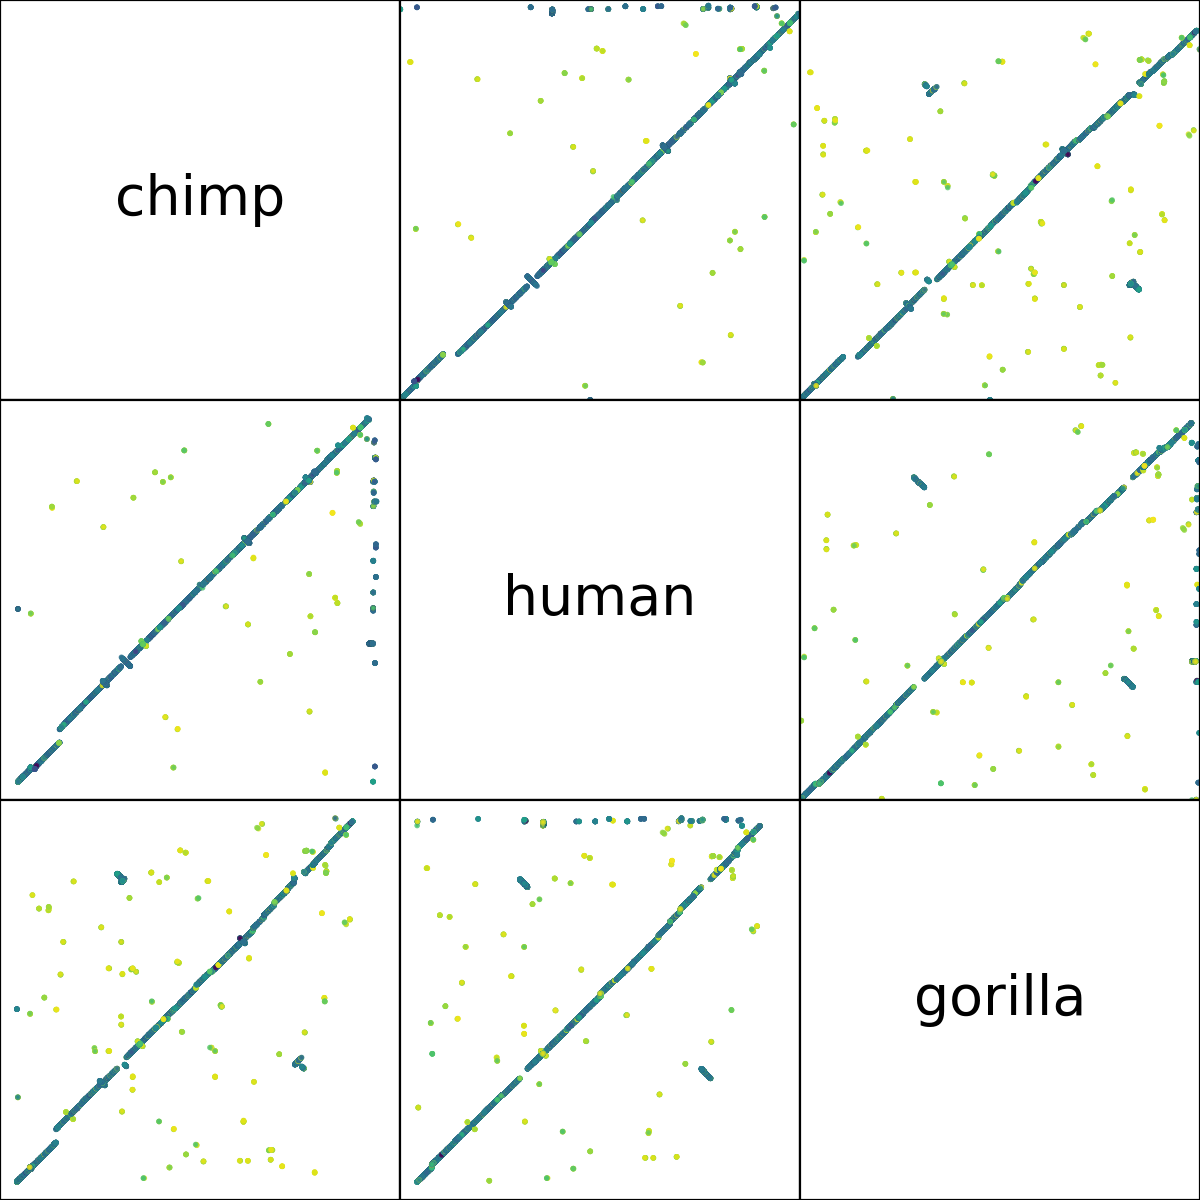
\includegraphics[width=0.48\columnwidth]{scatterplot_matrix_3}
 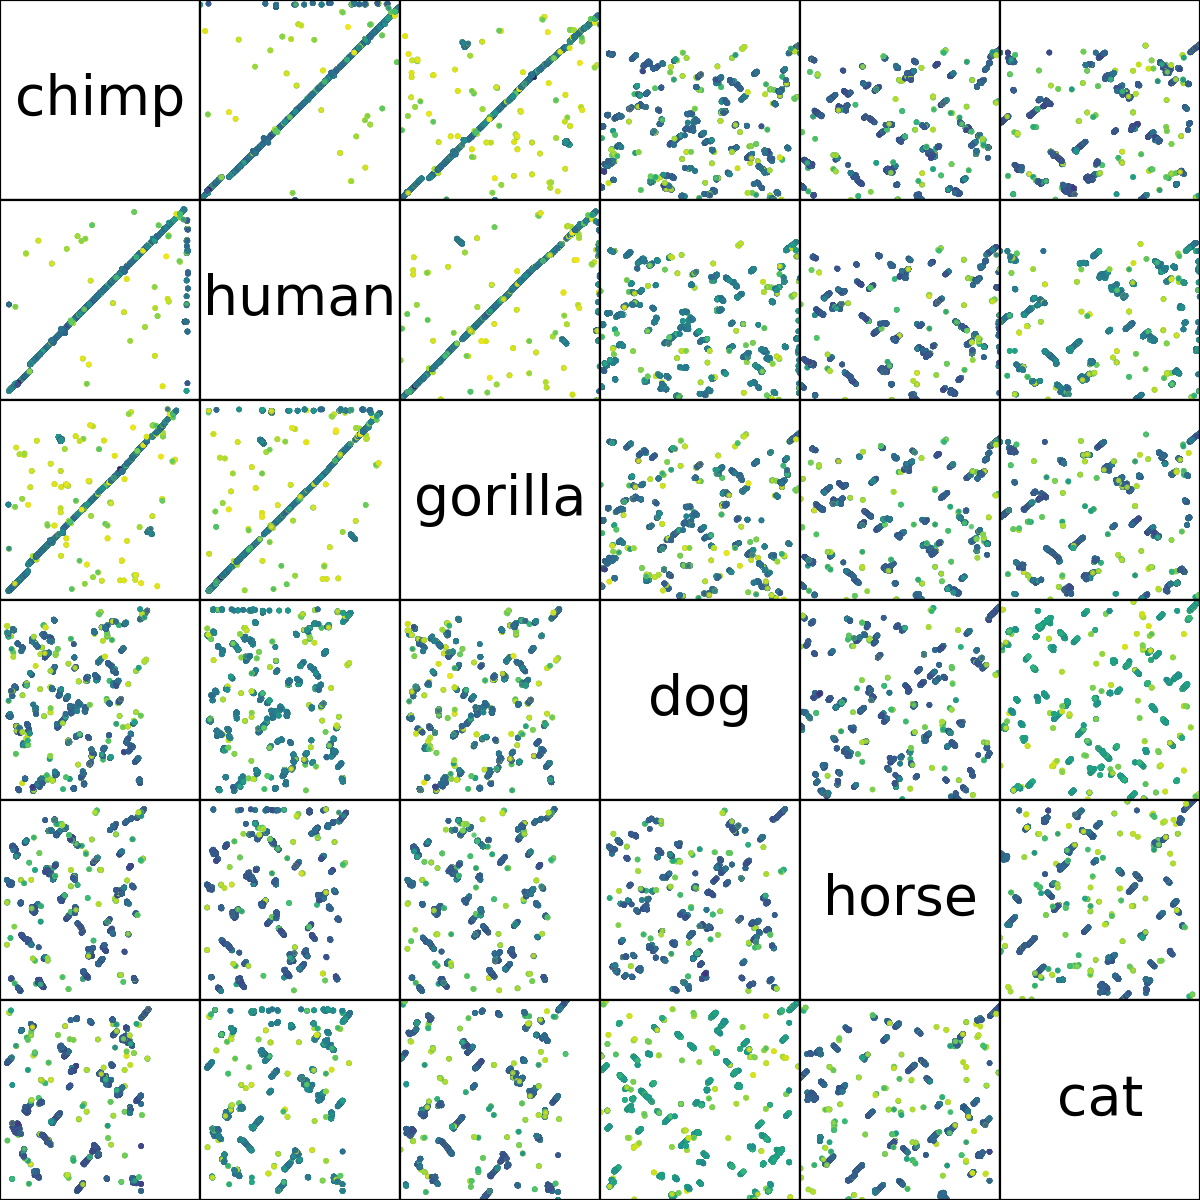
\includegraphics[width=0.48\columnwidth]{scatterplot_matrix_6}
 \caption{Two synteny matrix plots of three and six species respectively. Note that it becomes harder to inspect the relationship between genomes as the number of genomes involved increases.}
 \label{fig:synteny_matrices}
\end{figure}

\begin{figure}[t]
 \centering
 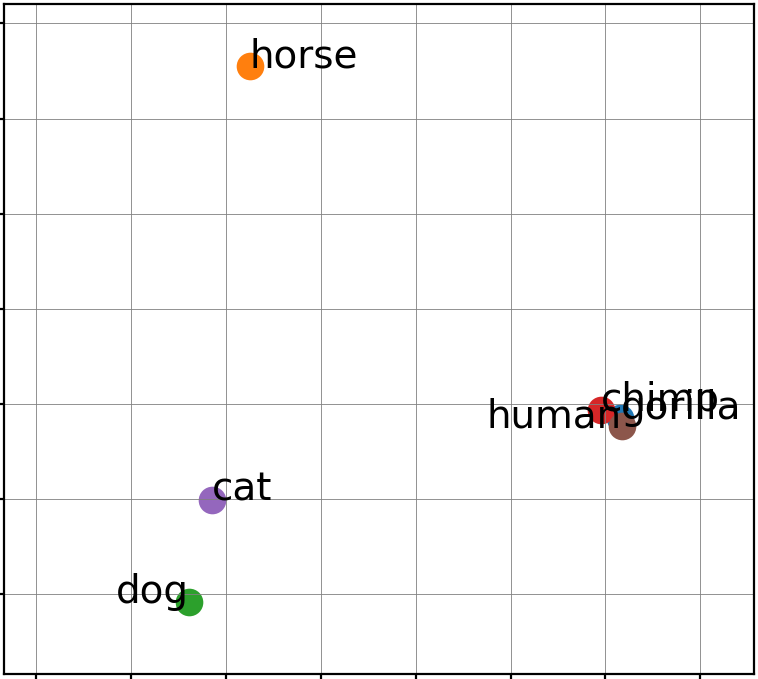
\includegraphics[width=0.48\columnwidth]{synmap_n}
 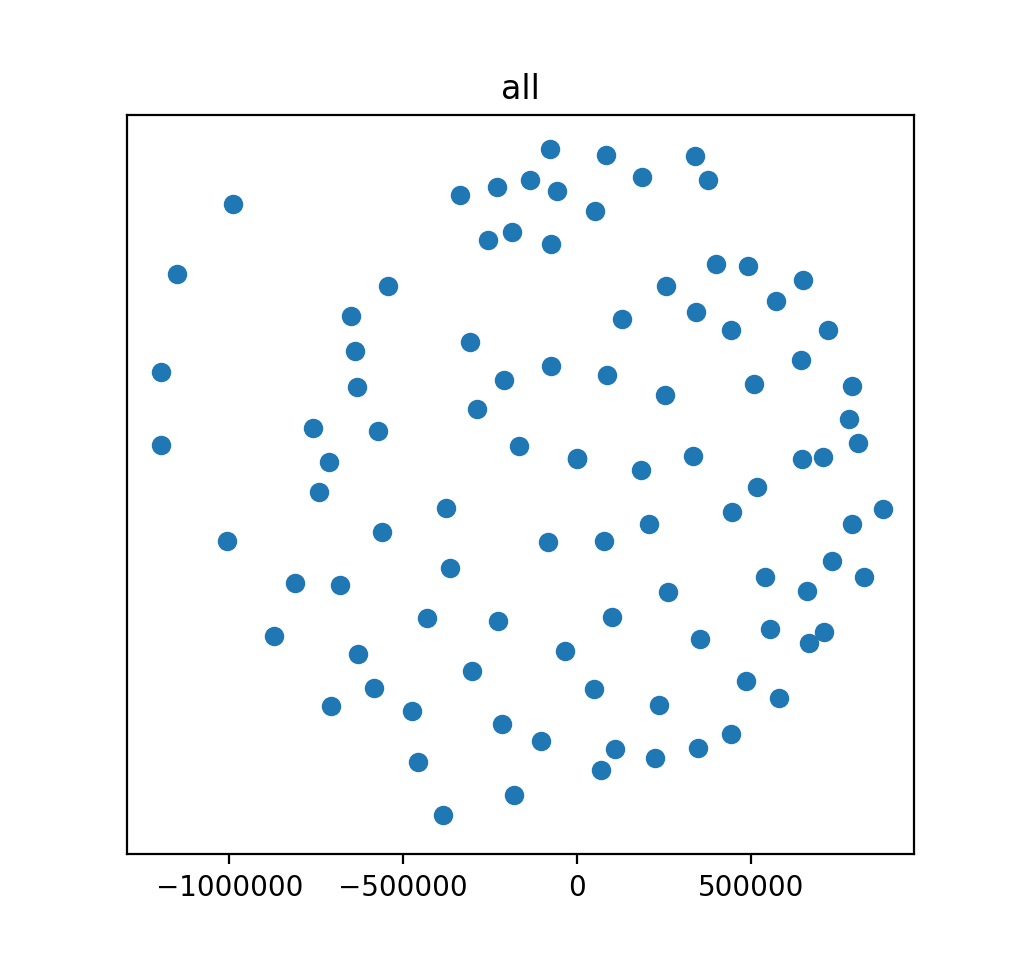
\includegraphics[width=0.46\columnwidth]{chr_all_scatter}
 \caption{With the notion of similarity between sets of genes we define, we can create a single plot that summarizes the similarities across genomes. Note that although this is helpful for the six-species plot on the left, this plot is not particularly helpful for the similarity comparison between the \emph{arabidopsis} genomes (on the right). We discuss this further in the text.}
 \label{fig:synmap_n}
\end{figure}

%% \begin{figure}[h]
%%  \centering
%%  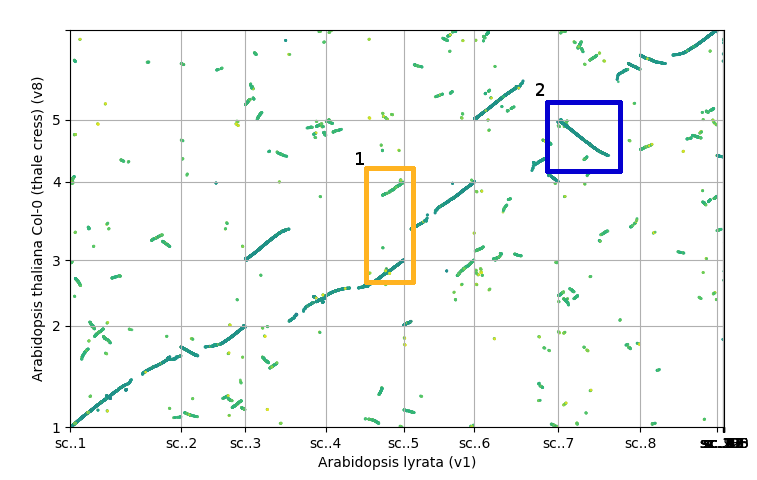
\includegraphics[width=0.8\columnwidth]{dotplot_arabidopsis_marked}
%%  \caption{A syntenic dotplot of Arabidopsis lyrata and Arabidopsis thaliana. The orange region 1 shows a duplication in Arabidopsis thaliana with respect to Arabidopsis lyrata. The blue region 2 shows an inversion. The image is regenerated by ks data downloaded from \cite{arabidopsisurl}.}
%%  \label{fig:dotplot_arabidopsis_marked}
%% \end{figure}

%\begin{figure}[h]
% \centering
% 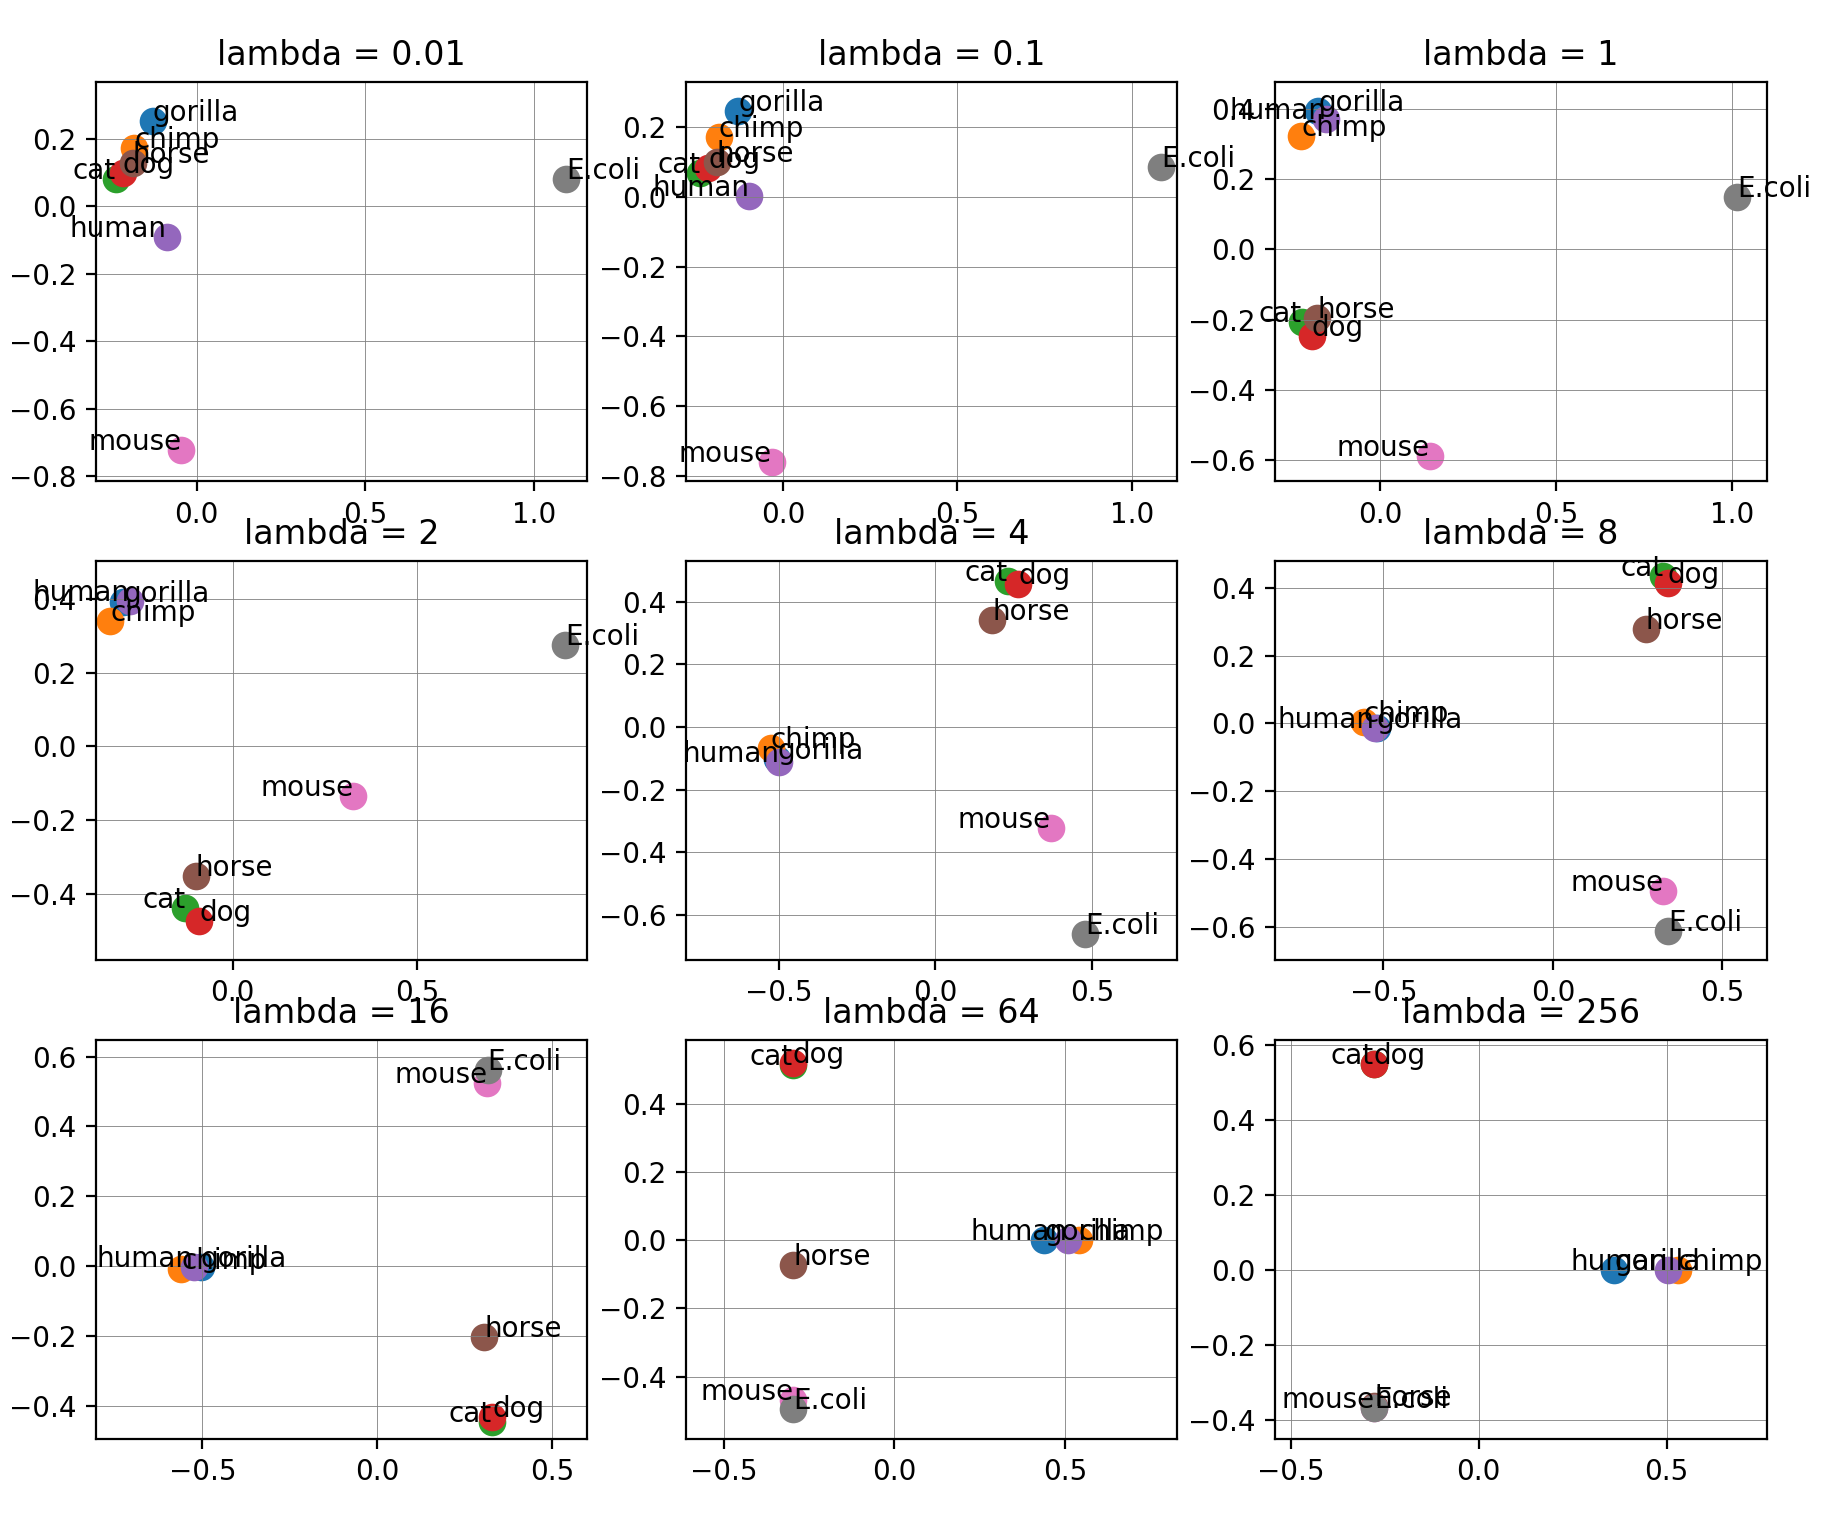
\includegraphics[width=\columnwidth]{lambda}
% \caption{lambda test}
% \label{fig:lambda}
%\end{figure}

 %TODO do this?
%\section{Related Works}
%% \section{Examples}
%% \autoref{fig:synmap_n} shows our first attempt of providing an overview of the genomes in concern. We define a similarity measure between two genomes, apply dimensionality reduction (Kernel PCA \cite{kernelpca}), and try to visualize the relationships among genomes of interest through a genomic map where distances between genomes encodes their affinity.

%% \begin{figure}[th]
%%  \centering
%%  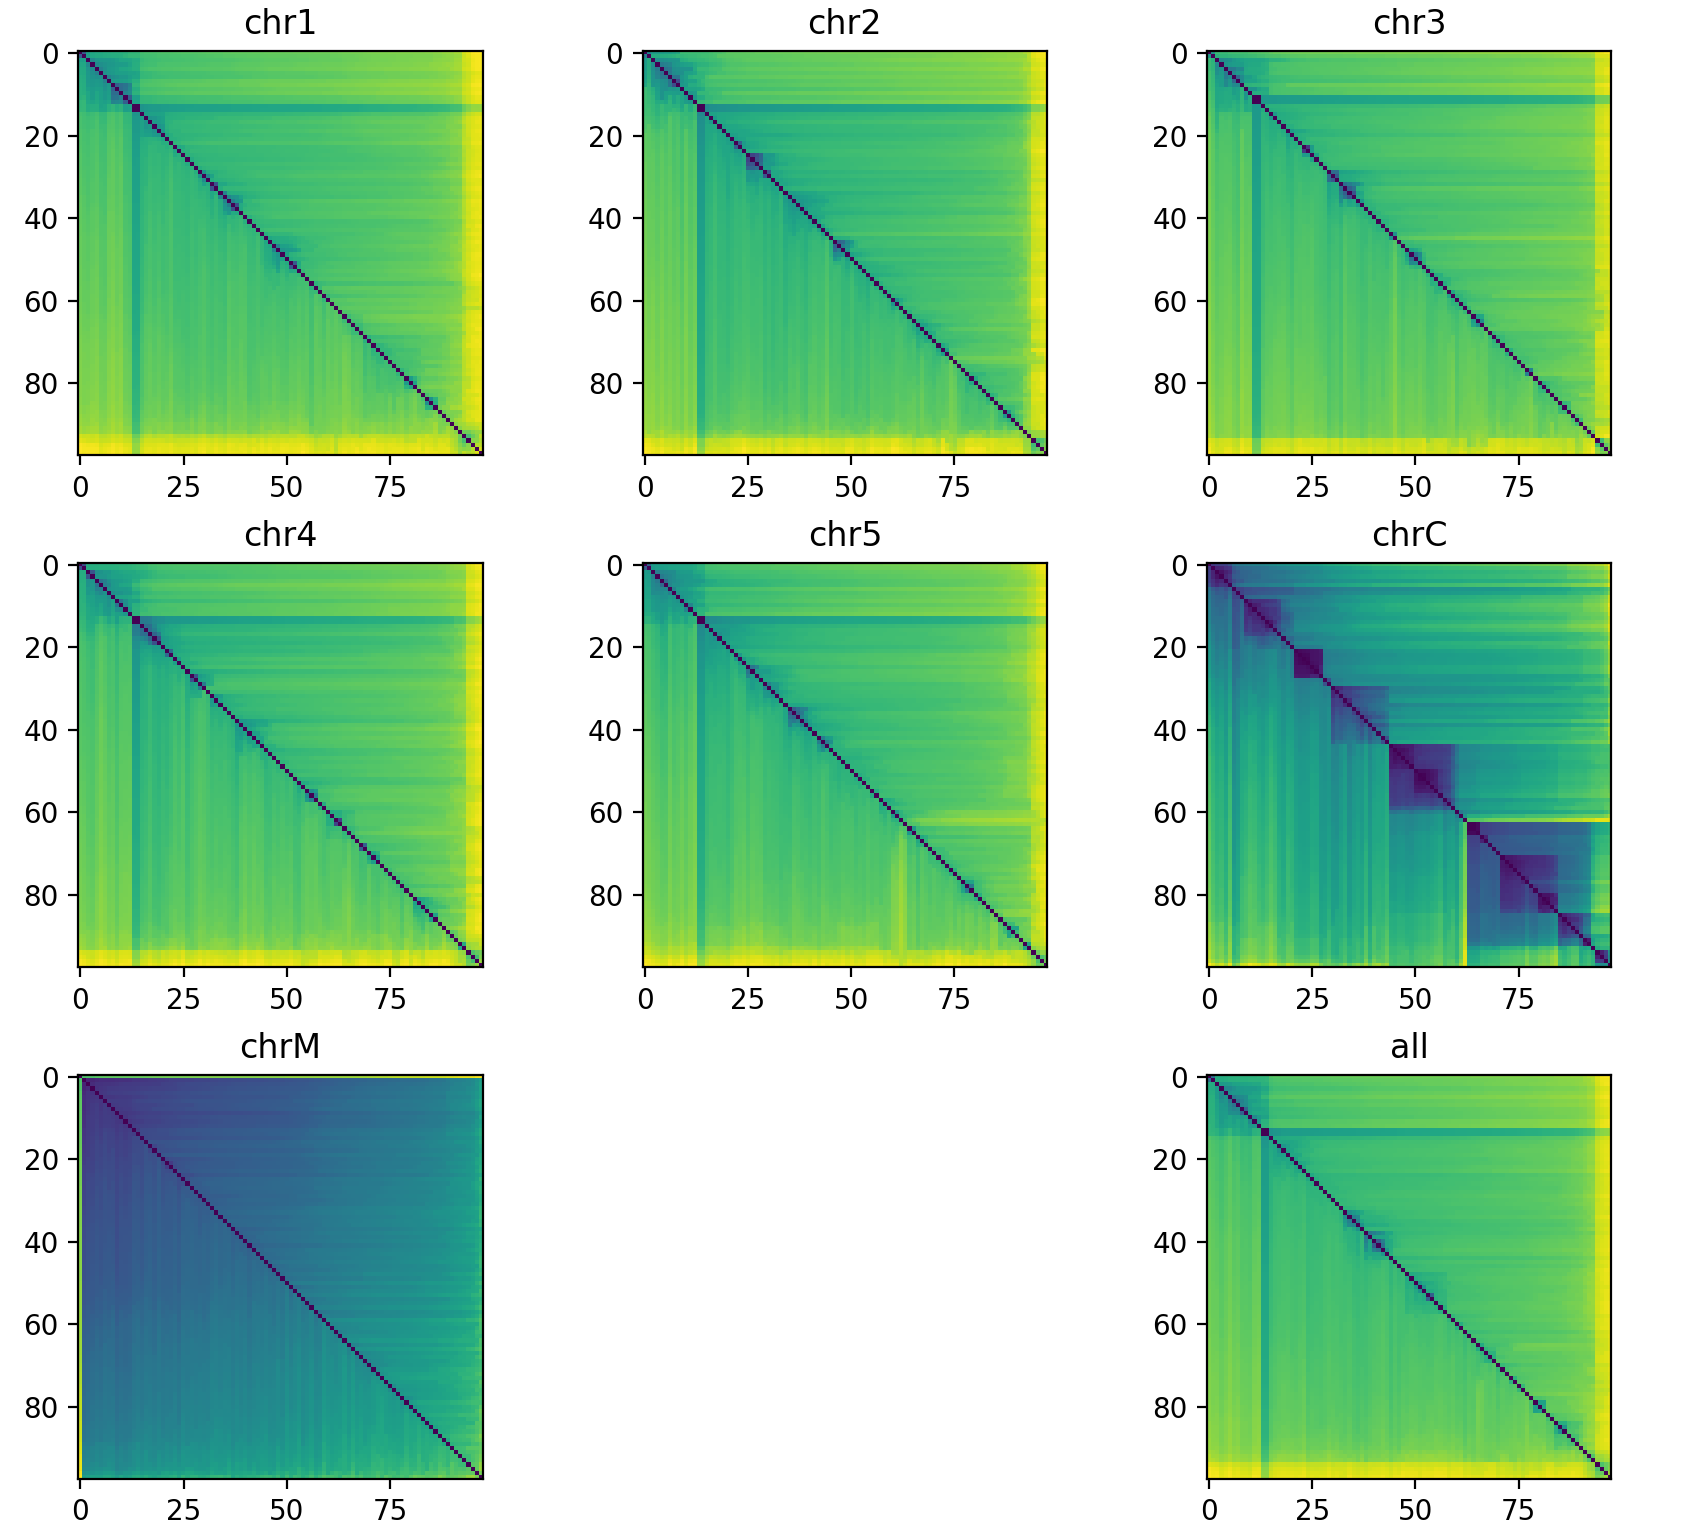
\includegraphics[width=0.8\columnwidth]{chromosomes_matrix}
%%  \caption{Distance matrices of 97 Arabidopsis thaliana of different ecotypes. Eight subplots are 7 individual chromosomes and a sum of them. Clusters and outliers can be spotted in chromosome C (subplot \#6)}
%%  \label{fig:chromosomes_matrix}
%% \end{figure}

%% \begin{figure}[th]
%%  \centering
%%  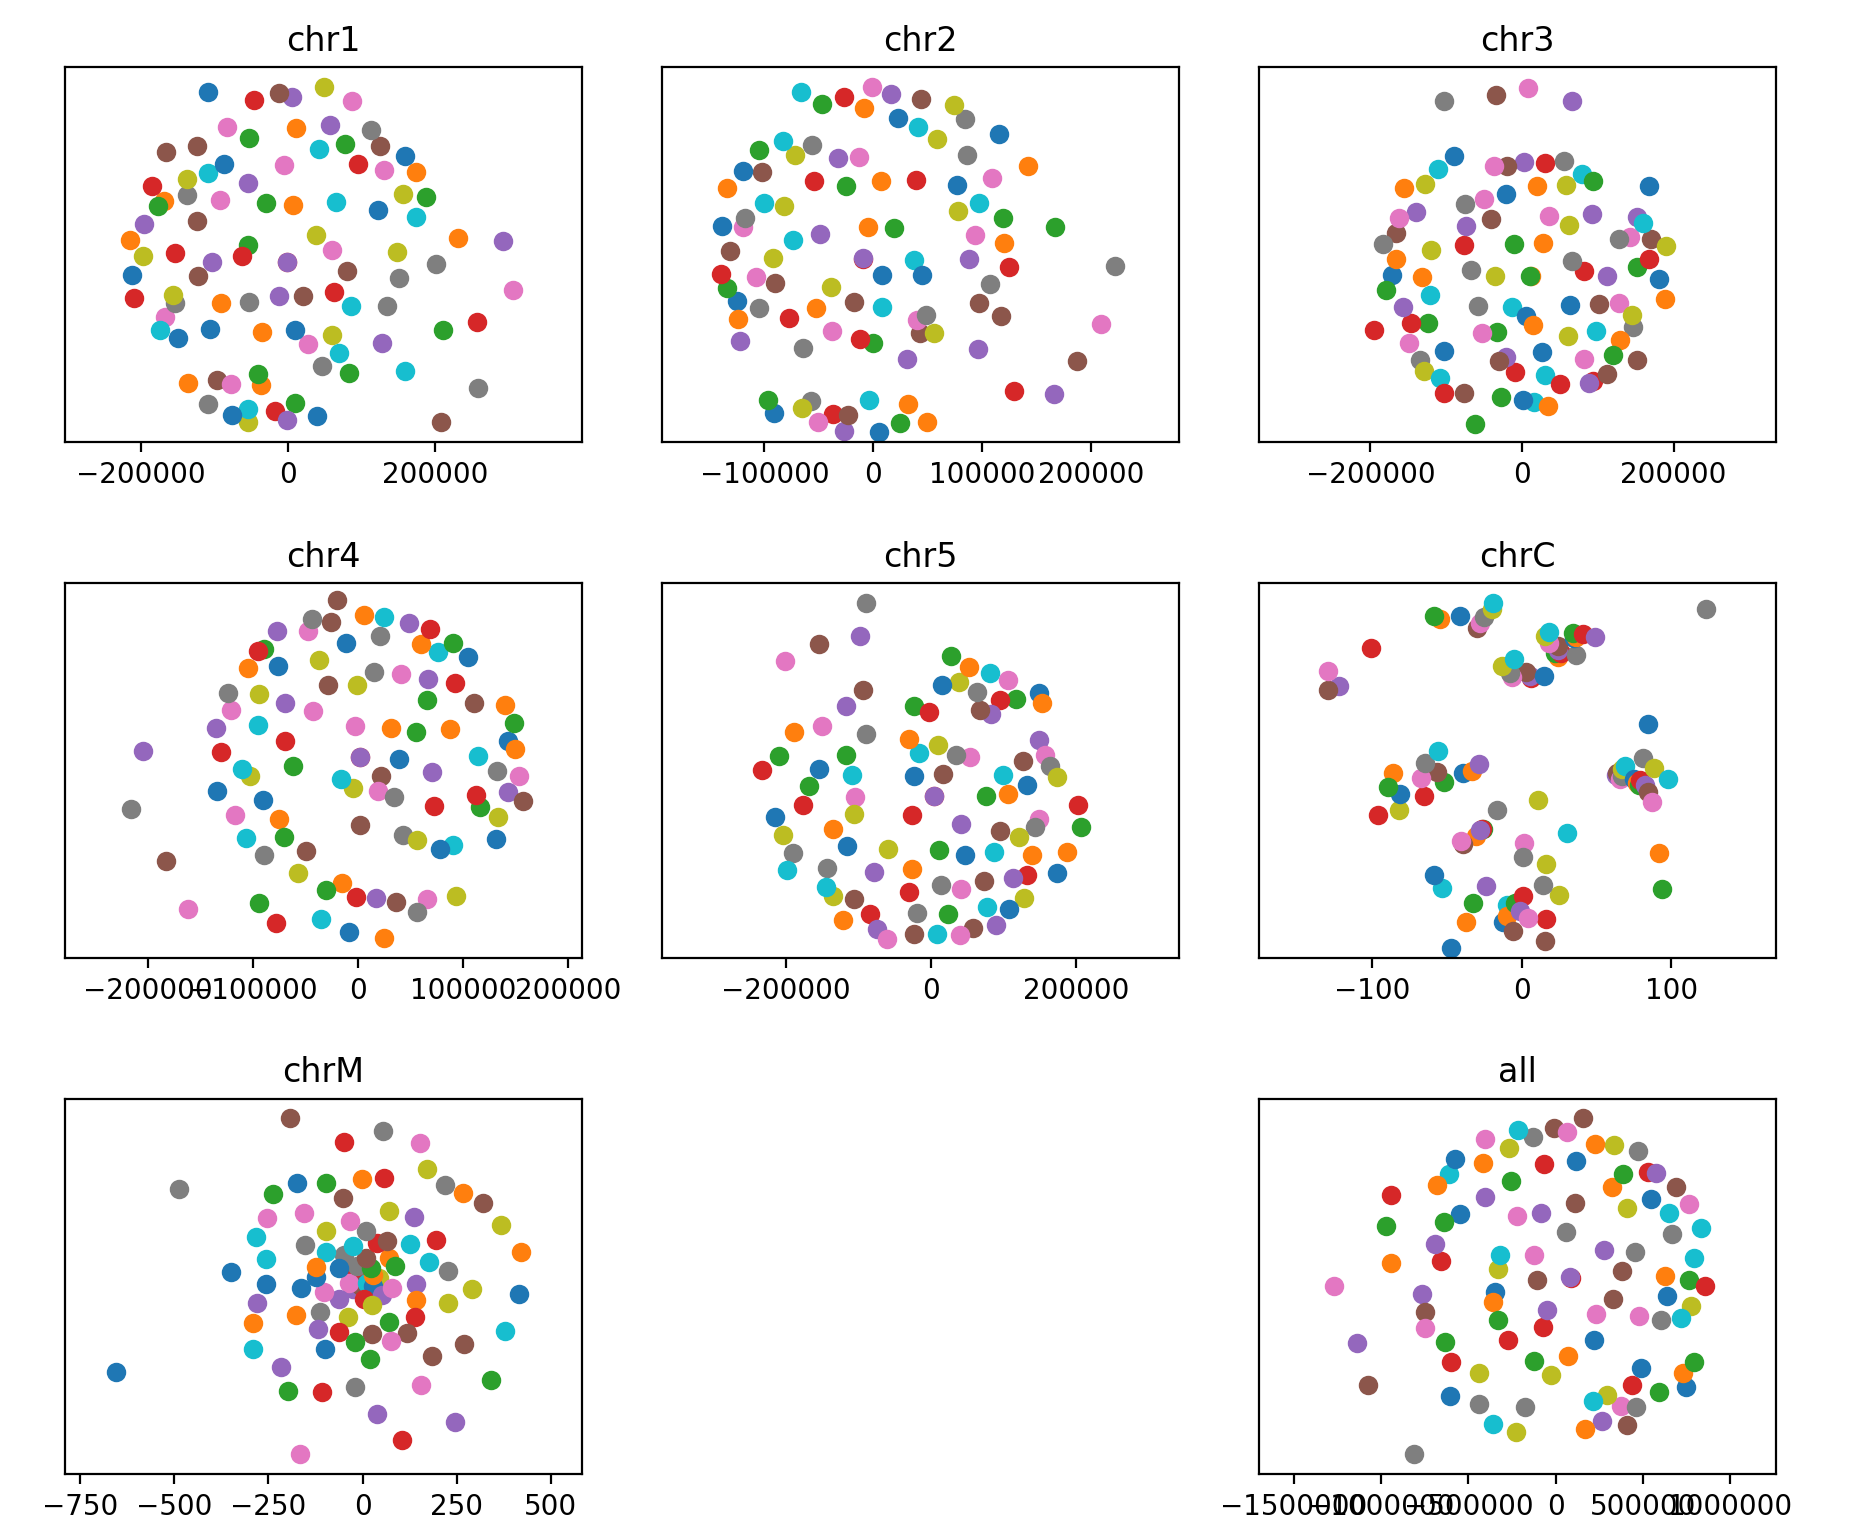
\includegraphics[width=0.8\columnwidth]{chromosomes_scatter}
%%  \caption{MDS plots of 97 Arabidopsis thaliana of different ecotypes.}
%%  \label{fig:chromosomes_scatter}
%% \end{figure}

%% \autoref{fig:chromosomes_matrix} and \autoref{fig:chromosomes_scatter} show distance matrices and scatterplots (coordinates computed from MDS) of species from another dataset. The genomes are Arabidopsis of different ecotypes. When we break the entire genome into individual chromosomes and try to compute their pairwise edit distances, we see clusters in small chloroplast chromosomes (chrC, subplot \#6 in \autoref{fig:chromosomes_matrix} and \autoref{fig:chromosomes_scatter}). We can also see some common outliers among other plots.

%TODO to be trimed
\section{Method}
In the process of generating a SynMap of two genomes, the synonymous mutation rate ($ks$ as described above) is computed for each pair of aligned genes between two genomes. This score ranges from $0$ to $+\infty$, or arbitrary large number in data, with $0$ means perfect alignment and infinity indicates no alignment or an error.
We want to utilize these measures to build a notion of distance between the two genomes (that is, between two \emph{sets} of genes).

%% For example, when comparing two genomes of human and chimp, we are given IDs of gene pairs and their synonymous mutation rate, denoted by $ks$, which can be seen as a measure of distance (\autoref{tab:table_input_example})
%% \begin{table}[h!]
%% \centering
%% \caption{Data Input File}
%% \label{tab:table_input_example}
%% \begin{tabular}{cc|c}
%% \toprule
%% %\multicolumn{2}{c}{Gene labels} &\\
%% %\midrule
%% Human & Chimpanzee & $ks_i$\\
%% gene ID & gene ID & \\
%% \midrule
%% h1 & c1 & 0.0056\\
%% h2 & c2 & 72.6574\\
%% ... & ... & ...	\\
%% \bottomrule
%% \end{tabular}
%% \end{table}

Now we want to find a function of all the $ks$ values that describe the distance between two genomes or, equivalently, a notion of similarity (or a ``kernel'') between the genomes.
%\begin{align}
%similarity(Human, Chimp) = g(ks_1,ks_2...)
%\end{align}
Generally, for any gene in one genome, there might be syntenic matches to more than one gene on the other genome. Computationally, this means we encode the similarity between the two genomes by arranging the $ks$ values in a matrix:

%ks_{2,1} & ks_{2,2} & ks_{2,3} & \dots & ks_{2, c}\\
%matrix representation
$$K = 
\begin{bmatrix}
ks_{1,1} & ks_{1,2} & \dots & ks_{1, c}\\
\vdots & \vdots & \ddots & \vdots \\
ks_{h,1} & ks_{h,2} & \dots & ks_{h, c}\\
\end{bmatrix},
$$

\noindent where $ks_{1,1}$ stores the $ks$ value between the first gene of human and the first gene of chimpanzee, and so on. The indices of rows and columns are in the order of gene locations in ordered chromosomes.
%, chromosomes are ordered in a natural order to genomicists. 
$h$ and $c$ are gene counts of human and chimpanzee respectively. One can think of $K$ as an image data of the SymMap plot. Now we want a function of $K$ that outputs a scalar value to describe the similarity between two genomes.
%\begin{align}
%similarity(Human, Chimp) = f(K)
%\end{align}

%TODO include this?
%Intuitively we want a measure similar to the dot product of vectors of unit length, which encodes cosine of the angle between the two vectors. Moreover, the dot products should better not generating any negative values since there is not a notion of 'negative of a human' among species.

To define a function so that comparison of a genome to itself gives a similarity measure close to $1$, we used $f$ to compute kernels between any two genomes, which are later used to plot \autoref{fig:synmap_n}
%f(K) = \frac{\sum_{i,j} e^{-\lambda K_{ij}}}{\sqrt{c \times h}}
\begin{align}
similarity(Human, Chimp) = f(K) = \sum_{i,j} e^{-\lambda K_{ij}}/\sqrt{c \times h}
\end{align}
Where $\lambda$ is a scalar constant related to sensitivity of the similarity measure. $c$ and $h$ are the gene counts defined before. 

Once we have the pairwise distances among multiple genomes (stored in matrix $M$), we have an implied space, which we can then project it onto a 2D screen using (for example) Kernel PCA.
%% Let $M$ be the matrix of similarities of multiple genomes where each entry is computed by function $f$ defined above. Note that this is a symmetric matrix with diagonal entries set to $1$, indicating complete identity in similarity measure of each genomes with respect to itself.
%% $$M = 
%% \begin{bmatrix}
%% f_{human, human} & f_{human, chimp} & f_{human,cat} & \dots \\
%% f_{chimp, human} & f_{chimp, chimp} & f_{chimp, cat} & \dots \\
%% \vdots & \vdots & \vdots & \ddots \\
%% \end{bmatrix}
%% $$
%% We then treat it as a kernel matrix and feed it into existing Kernel PCA algorithms and plot the first two principle components, which is shown in \autoref{fig:synmap_n}
One example of this technique being used can be seen in \autoref{fig:synmap_n}.

The definition above works for general comparisons between genomes whose differences are encoded with syntenic matches.
In the case of genome differences encoded through sets of SNPs, we use a simpler definition of distances, based entirely on comparing the nucleotide polymorphisms and counting their differences.

\section{Limitations and ongoing work}

SynMapN gives an overview of genomes, but the detailed patterns within two genomes such as inversions and duplications are not visible.
As can be clearly seen on the right side of \autoref{fig:synmap_n}, the dimensionality reduction plots break down for large numbers of genomes. In addition (and in contrast to the SynMap plots) they provide little insight about \emph{what} causes the genomes to be different. In our ongoing collaboration, we are developing tools that will provide the level of detail present in syntenic dotplots, with the visual scalability of dimensionality reduction plots. Consider, for example, a breakdown of the \emph{arabidopsis} genome differences with respect to different chromosomes, as shown in~\autoref{fig:per-chromosome}. Especially in settings where genomic differences are complex and structural in nature (\autoref{fig:plasmodium}), the current dimensionality reduction plot will be not be sufficient.

\begin{figure}[t]
 \centering
 %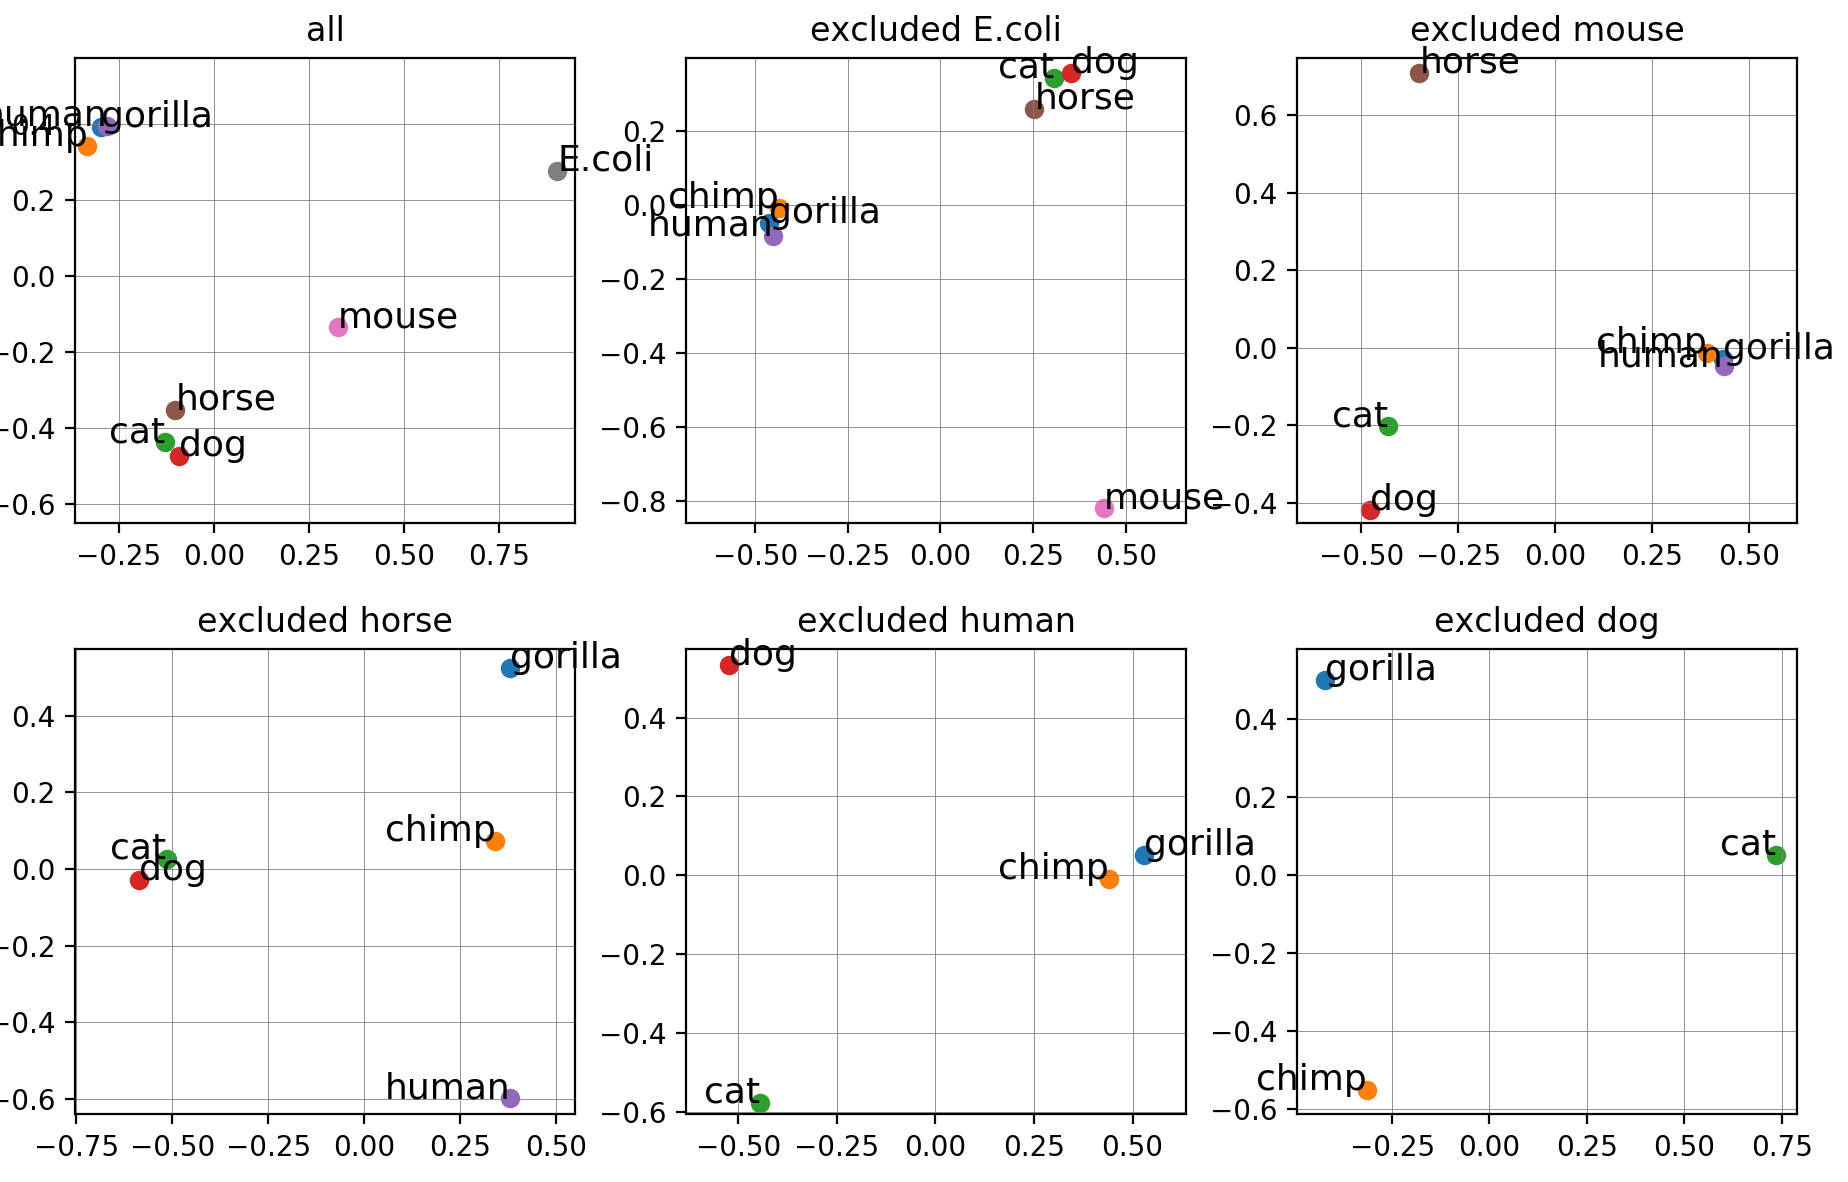
\includegraphics[width=0.8\textwidth]{subset}
 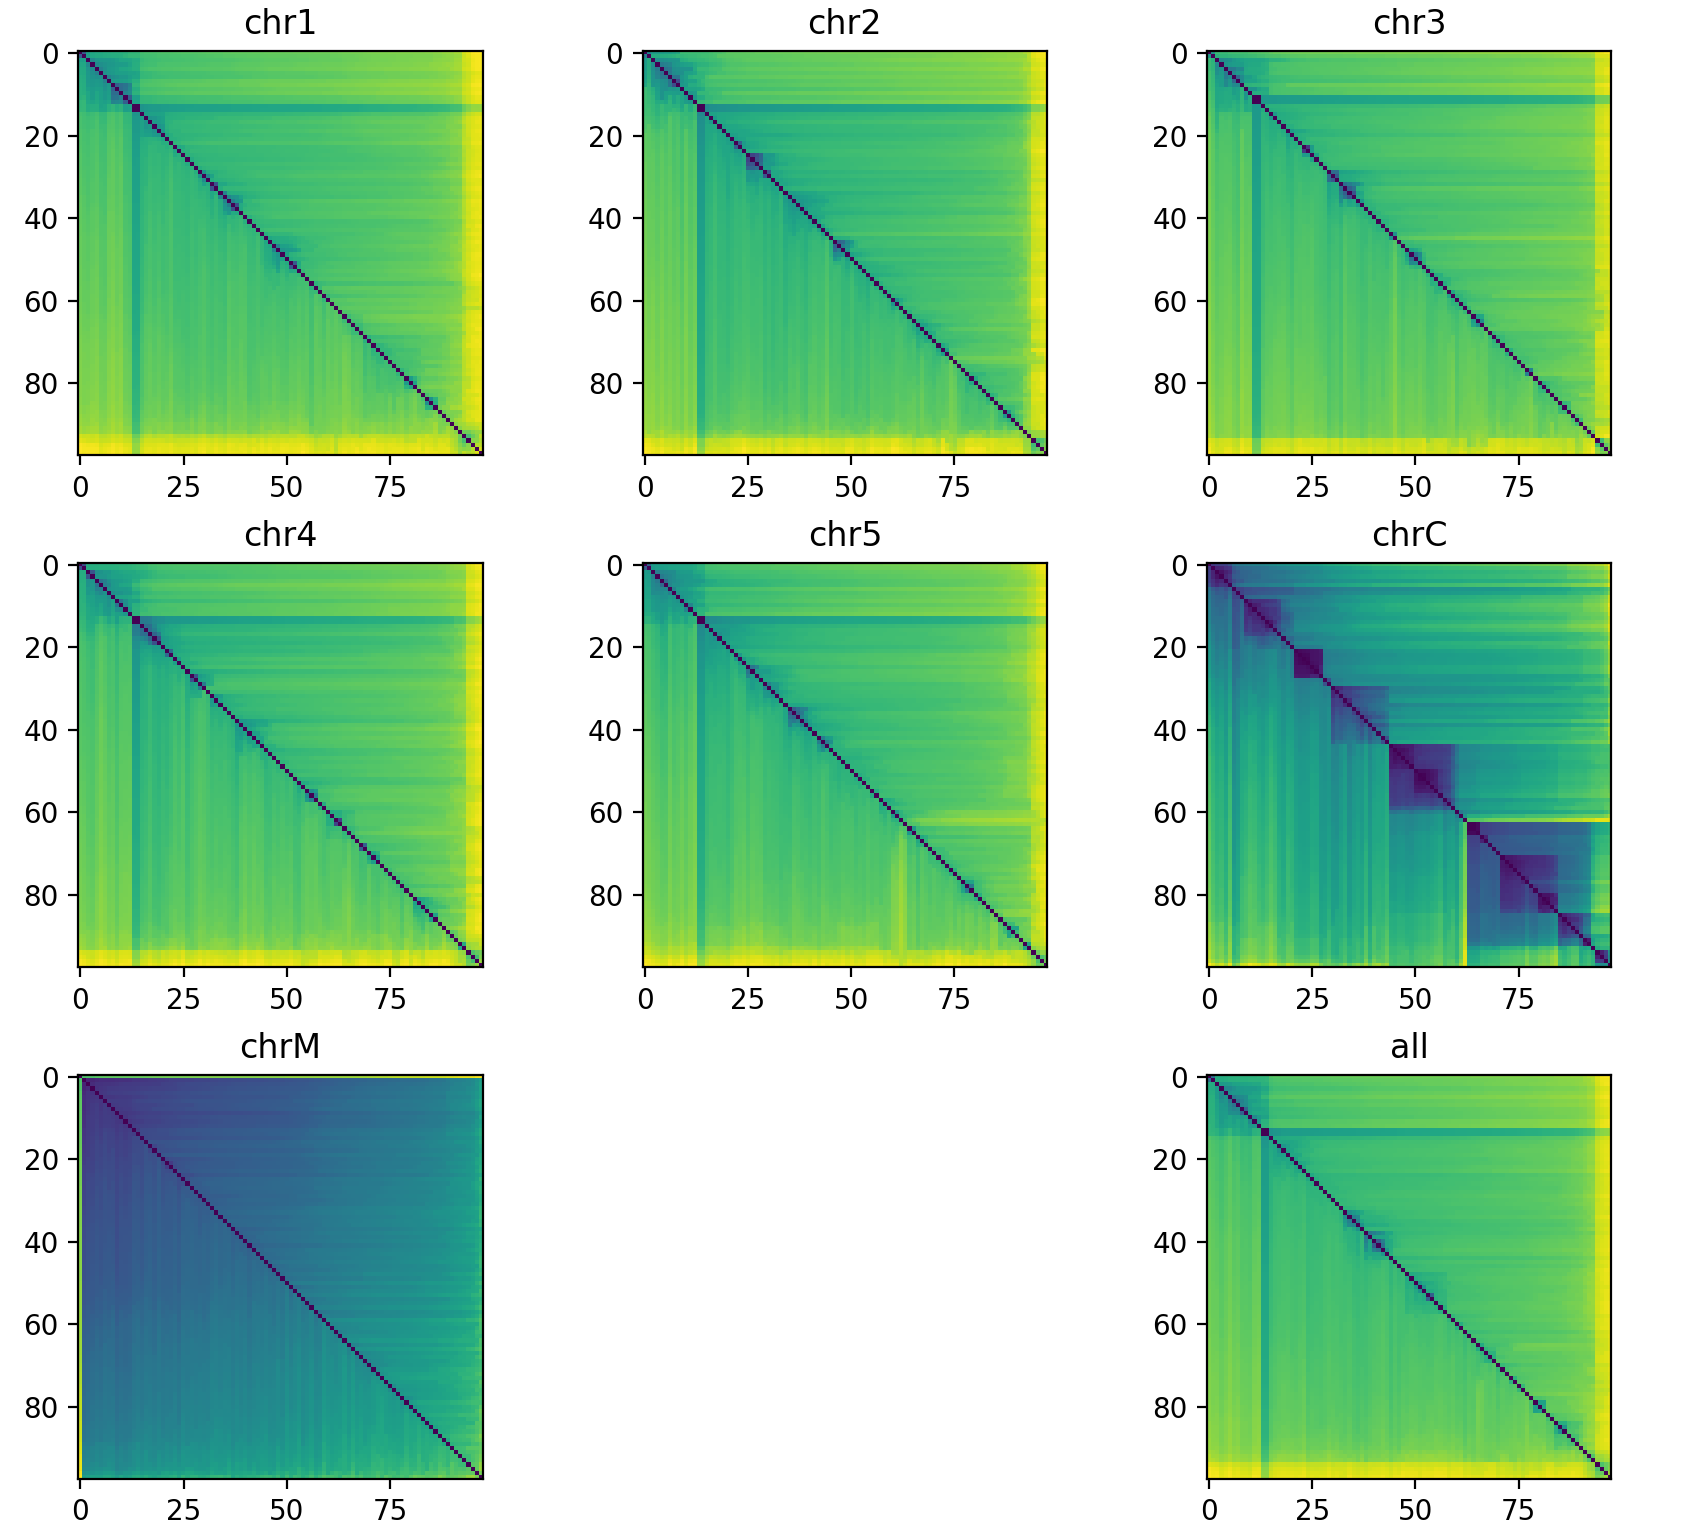
\includegraphics[width=\columnwidth]{chromosomes_matrix}
 \caption{A matrix plot of the genomic differences broken down by chromosome. Note the difference in variability across different chromosomes (specifically the genome in the chloroplast, encoded as ``chromosome C''). We are currently developing tools to help genomicists to better understand these differences.}
 \label{fig:per-chromosome}
\end{figure}

\begin{figure}[t]
 \centering
 %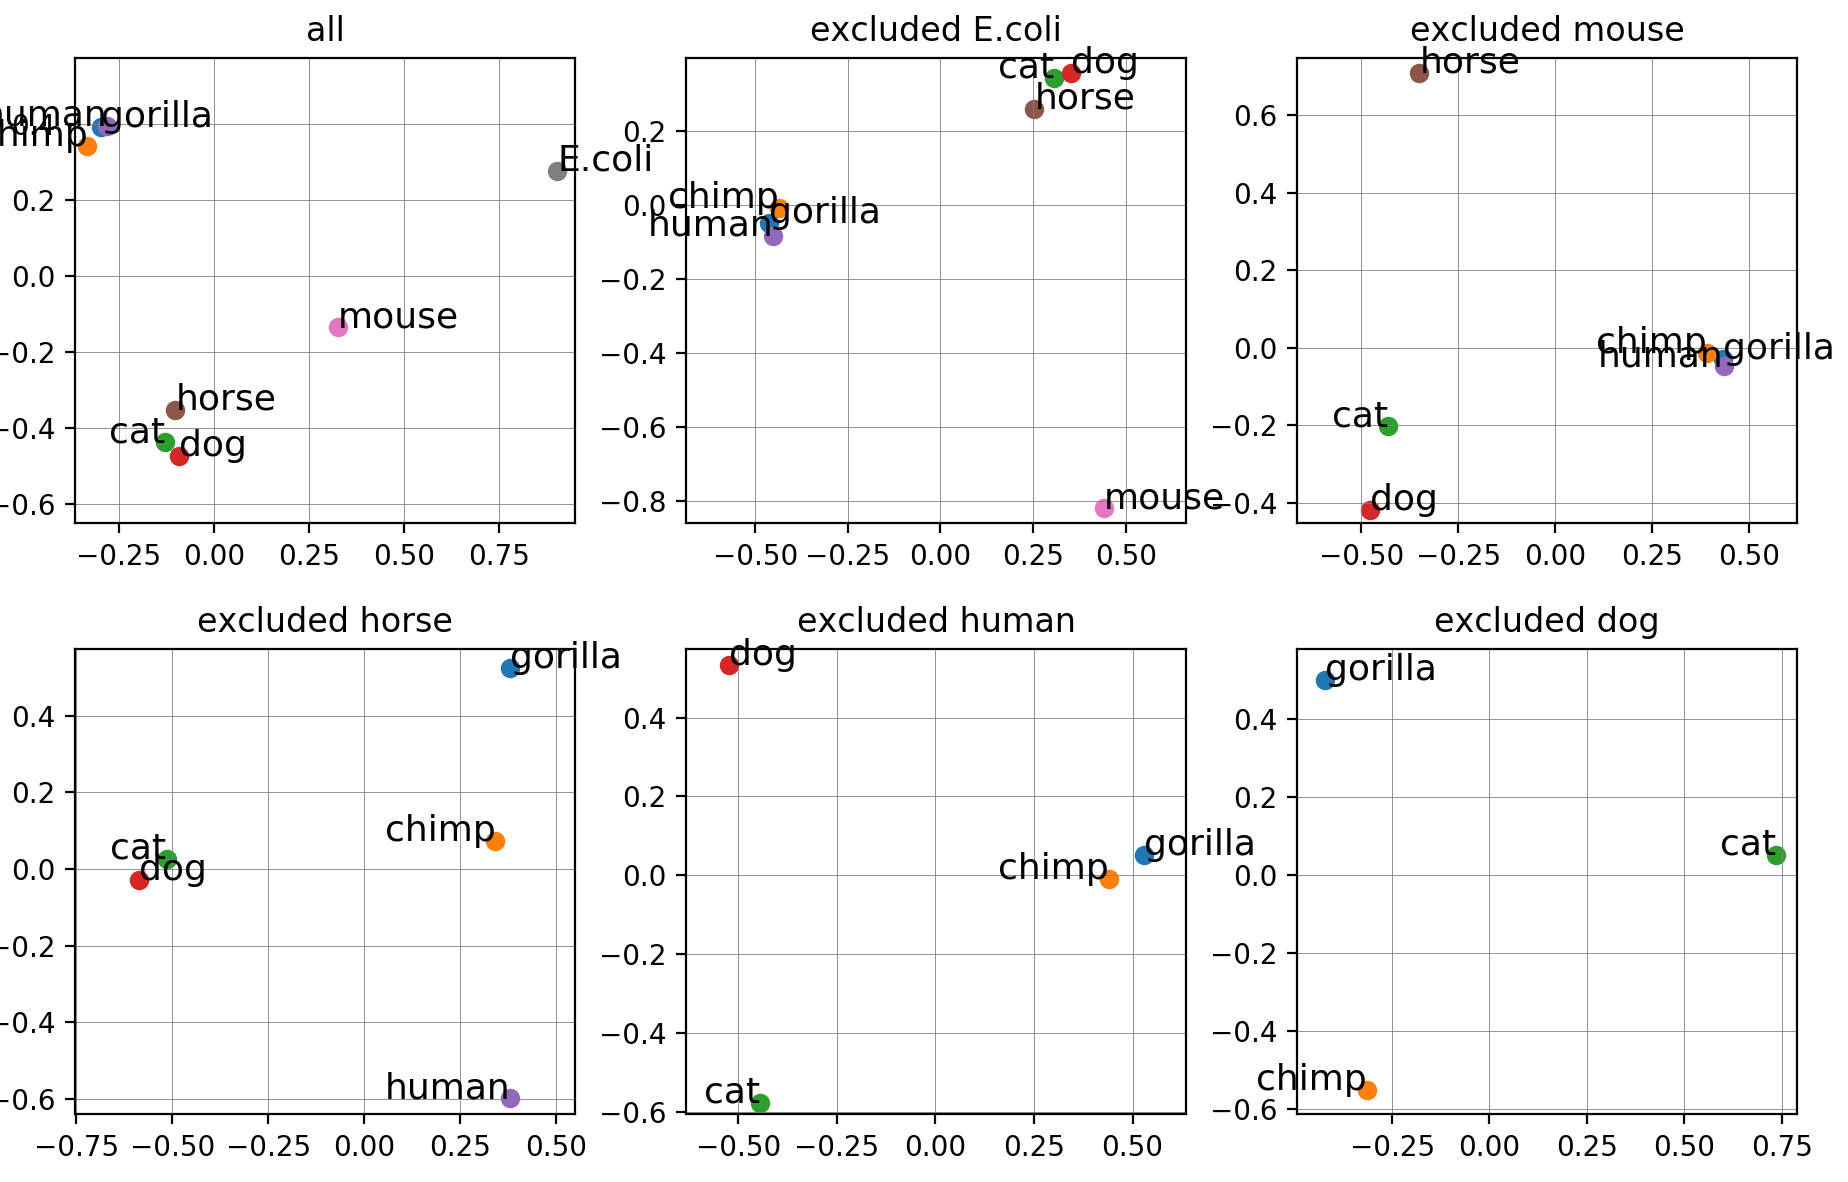
\includegraphics[width=0.8\textwidth]{subset}
 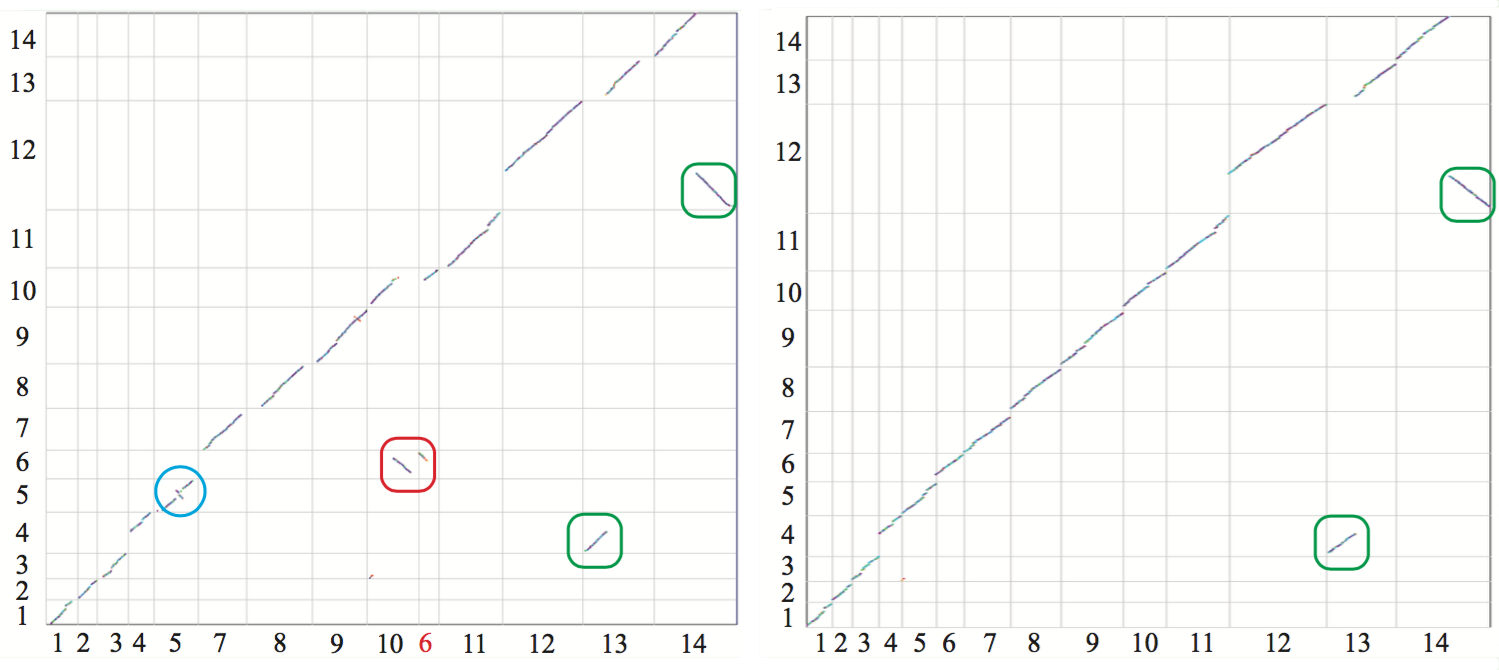
\includegraphics[width=0.6\columnwidth]{plasmodium}
 \caption{In cases where the task involves complex genomic differences such as the ones in our \emph{plasmodium} genome comparison use case shown here, currently-available techniques are not sufficient. Even though in this figure we show only two syntenic dot plots, the use case involves a total of 136 different comparisons, and that requires the development of novel tools and techniques.}
 \label{fig:plasmodium}
\end{figure}


%% In addition to the example plot in \autoref{fig:synmap_n}, we explore different subsets of the genomes among the genomes we concerned to show the capacities and constraints of SynMapN. 
%We show another distance measure used for a different dataset of more similar species represented in single-nucleotide polymorphism (SNP) data format.

%different lambda values and diferent subset of genomes
%closely related genomes, different approach

%(more on SNPs dataset?)
  
In a complete visualization system, we expect to enable users to navigate through various visualizations for different levels of details, from high level SynMapN to very detailed comparison of two specific genomes in SynMap. To further increase the number of levels, we can split genomes into individual chromosomes and compare them in SymMapN. We are also exploring the possibilities of capturing certain features in a SynMap plot, for example, the diagonal alignments or anti-diagonal alignments, using image processing techniques. More improvements on interaction can be done through studying observation level interactions \cite{endert2011observation}, to enable users to specify desired clustering criteria through dragging points in the plot. 

%TODO do this?
%\section{Conlcusion}



%% if specified like this the section will be committed in review mode
%\acknowledgments{
%The authors wish to thank A, B, C. This work was supported in part by
%a grant from XYZ.
%}

%\bibliographystyle{abbrv}
\bibliographystyle{abbrv-doi}
%\bibliographystyle{abbrv-doi-narrow}
%\bibliographystyle{abbrv-doi-hyperref}
%\bibliographystyle{abbrv-doi-hyperref-narrow}

\bibliography{mybib}
\end{document}
